\chapter{Correlation of \diiid's toroidally separated interferometers}
The toroidal structure of an MHD mode can strongly influence
the mode's stability and its interaction with the surrounding plasma.
A mode's toroidal structure is typically characterized
via the toroidal mode number $n$.
Historically, measurement of toroidal (and poloidal) mode numbers
with magnetic loops has provided rich insight
into the physics governing numerous operational regimes and stability limits.
However, core-localized MHD produces weak signals outside of the plasma volume,
making measurement of mode numbers via magnetic loops difficult or impossible.
Recently, measurements from toroidally separated
electron cyclotron emission imaging (ECEI) systems
on the KSTAR tokamak have identified mode numbers of
edge-localized modes~\cite{lee_rsi_2014} and
sawteeth~\cite{choe_nf_2015},
raising the question as to the utility of using more exotic measurements
to probe the structure of core-localized MHD.

This chapter describes the use of toroidally separated interferometers
to measure toroidal mode numbers.
To the author's knowledge, this is the first such implementation in a tokamak.
The addition of the heterodyne interferometer channel
to \diiid's pre-existing phase contrast imaging (PCI) system
enabled this novel measurement.
As shown in Fig.~\ref{fig:ToroidalCorrelation:pci_interf_locs}
the beampaths of the PCI and V2 interferometers
are toroidally separated by $\Delta \zeta = 45^{\circ}$ and
are very nearly radially overlapping.
Section~\ref{sec:ToroidalCorrelation:two_point_correlations}
reviews the mathematics of the two-point-correlation technique
used to extract toroidal mode numbers and
derives the resulting Nyquist mode number.
Section~\ref{sec:ToroidalCorrelation:interferometer_measurements}
examines the interferometer measurements in detail and
develops a formula for the measured toroidal mode number.
Section~\ref{sec:ToroidalCorrelation:nonideal_effects}
characterizes the effects of time-base offsets and radial offsets
between the two interferometer systems and
describes methods to minimize their influence
on the measured toroidal mode number.

\begin{figure}
  \centering
  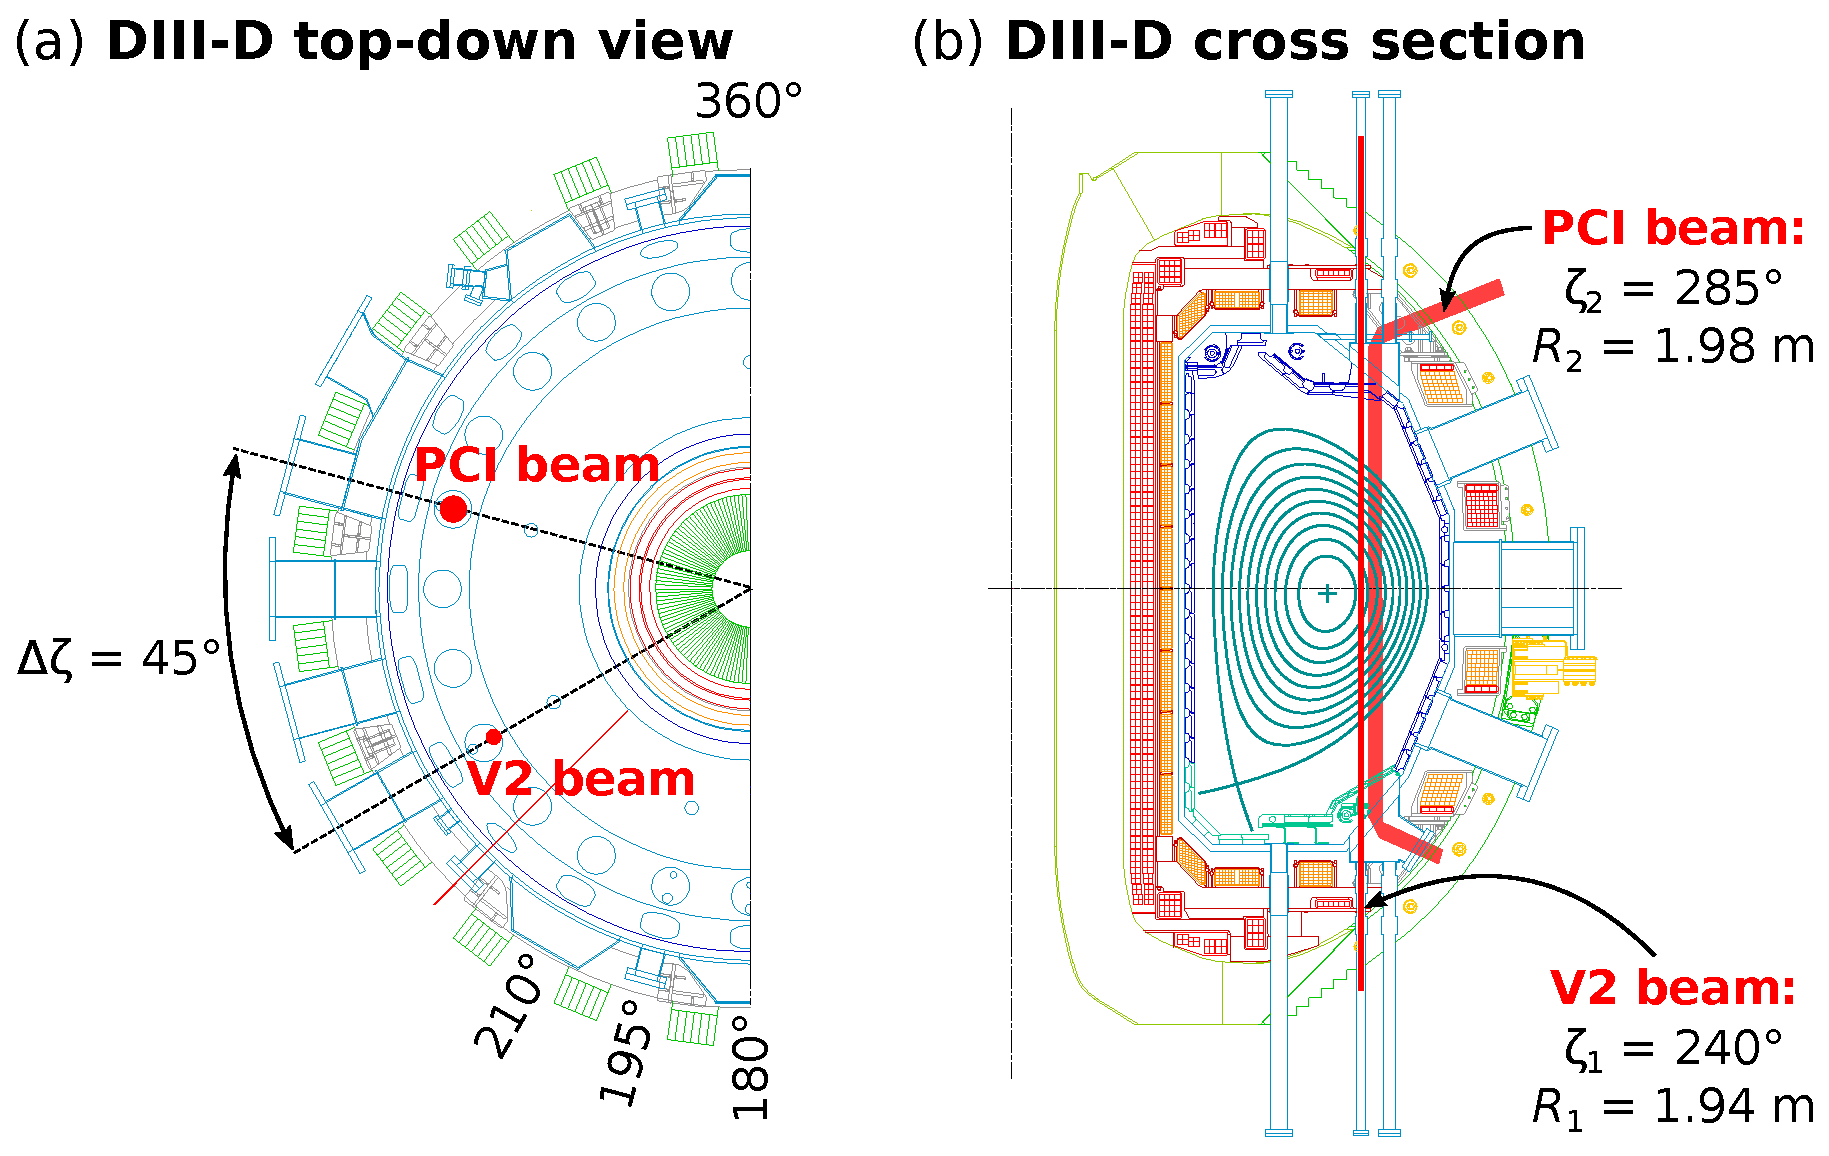
\includegraphics[width = \textwidth]{%
    Chapters/ToroidalCorrelation/figs/pci_interf_locs.eps}
  \caption[Beam locations of the V2 interferometer and PCI systems on \diiid]{%
    (a) A top-down view of the \diiid\space vessel.
    The V2 interferometer beam's toroidal location is $\zeta_1 = 240^{\circ}$,
    and the PCI beam's toroidal location is $\zeta_2 = 285^{\circ}$.
    (b) A view of the \diiid\space cross section.
    The V2 interferometer beam's
    major-radial location is $R_1 = \SI{1.94}{\meter}$, and
    the PCI beam's major-radial location is $R_2 = \SI{1.98}{\meter}$.}
\label{fig:ToroidalCorrelation:pci_interf_locs}
\end{figure}


\section{Two-point correlations}
\label{sec:ToroidalCorrelation:two_point_correlations}


\subsection{Spectral characterization of random processes}
In contrast to deterministic processes,
random processes cannot be modeled via an explicit mathematical relationship.
Rather, random processes are characterized
in terms of probabilities and statistical properties.
Any given observation of a random process represents
only one of many possible observations;
each such observation is referred to as
a ``sample'' or a ``realization'' of the random process
and is denoted as $x_k(t)$.
The random process itself consists of
the ensemble of all of the potential observations
and is denoted as $\{x_k(t)\}$.
Random processes can be stationary or nonstationary.
The statistical properties of a stationary random process
do not vary in time, and
the spectral tools discussed below
were all developed for analysis of stationary random processes.

The \emph{finite} Fourier transform $X_k(f, T)$
of a continuous signal $x_k(t)$ is defined as
\begin{equation}
  X_k(f, T)
  =
  \int_{-T / 2}^{T / 2}
  dt \, x_k(t) e^{-i \, 2 \pi f t}
  \label{eq:ToroidalCorrelation:finite_Fourier_transform}
\end{equation}
Note that $x_k(t)$ need \emph{not} be integrable over the infinite domain,
making the finite Fourier transform a suitable tool for stationary signals,
whose statistical properties (e.g.\ mean, variance, etc.) are
constant and potentially finite in time.

For real-valued, stationary random processes $\{x_k(t)\}$ and $\{y_k(t)\}$,
the one-sided cross-spectral density function $G_{xy}(f)$ is defined as
\begin{equation}
  G_{xy}(f)
  \equiv
  \lim_{T \rightarrow \infty}
  \frac{2}{T} E \left[ X_k^*(f, T) Y_k(f, T) \right]
  \label{eq:ToroidalCorrelation:cross_spectral_density_defn}
\end{equation}
for $0 < f < \infty$;
$G_{xy}(f)$ is not defined for $f < 0$, and
it is reduced by a factor of two relative to
(\ref{eq:ToroidalCorrelation:cross_spectral_density_defn}) at $f = 0$
(the value of $G_{xy}(0)$ is of little relevance to this work).
Note that $E[\cdot]$ is the expectation value operator;
this operator averages over all of the realizations in the ensemble, and
its application ensures that
(\ref{eq:ToroidalCorrelation:cross_spectral_density_defn})
is a statistically consistent definition of the cross-spectral density
(that is, ensemble averaging is needed for $G_{xy}(f)$
to approach the true cross-spectral density as $T \rightarrow \infty$).
In general $G_{xy}(f)$ is a complex-valued function;
this can be explicitly written as
\begin{equation}
  G_{xy}(f) = \left| G_{xy}(f) \right| e^{i \theta_{xy}(f)}
  \label{eq:ToroidalCorrelation:cross_spectral_density_explicit_complex}
\end{equation}
where $\theta_{xy}(f)$ is the \emph{phase angle}.
For the special case $\{x_k(t)\} = \{y_k(t)\}$,
$G_{xx}(f)$ is real-valued (i.e.\ $G_{xx}(f) = |G_{xx}(f)|$) and
is referred to as the one-sided autospectral density function.

The degree of correlation between random processes
$\{x_k(t)\}$ and $\{y_k(t)\}$ can be easily quantified
with the corresponding spectral density functions.
In particular, the magnitude-squared coherence function
$\gamma_{xy}^2(f)$ is defined as
\begin{equation}
  \gamma_{xy}^2(f)
  \equiv
  \frac{|G_{xy}(f)|^2}{G_{xx}(f) G_{yy}(f)}
  \label{eq:ToroidalCorrelation:magnitude_squared_coherence_defn}
\end{equation}
and it satisfies
\begin{equation}
  0 \leq \gamma_{xy}^2(f) \leq 1
  \label{eq:ToroidalCorrelation:magnitude_squared_coherence_bounds}
\end{equation}
for $0 \leq f < \infty$, with
$\gamma_{xy}^2(f) = 1$ indicating that
$\{x_k(t)\}$ and $\{y_k(t)\}$ are 100\% correlated at frequency $f$ and
$\gamma_{xy}^2(f) = 0$ indicating that
$\{x_k(t)\}$ and $\{y_k(t)\}$ are completely uncorrelated at frequency $f$.
Note that the ensemble-averaging operation in
(\ref{eq:ToroidalCorrelation:cross_spectral_density_defn})
is paramount to the computation
of \emph{informative} values for $\gamma_{xy}^2(f)$;
that is, if ensemble averaging is ignored, and
only single realizations of the random processes are used,
$\gamma_{xy}^2(f) \equiv 1$ for all $f$,
\emph{regardless} of the actual degree of coherence
between between $\{x_k(t)\}$ and $\{y_k(t)\}$.

Care should be taken when computing spectral densities.
In various programming languages,
it is not uncommon to ``detrend'' realizations $x_k(t)$ and $y_k(t)$
by subtracting the signal mean or linear trend
prior to application of
(\ref{eq:ToroidalCorrelation:cross_spectral_density_defn}).
However, the author has empirically found that
such detrending can lead to values of $\gamma_{xy}^2(f)$
that unphysically exceed the bounds established in
(\ref{eq:ToroidalCorrelation:magnitude_squared_coherence_bounds}).
The author has not explored more exotic means of detrending, and
no detrending was applied to signals prior to spectral computations
in this work.


\subsection{Nyquist mode number}


\section{Toroidal correlation of interferometers}
\label{sec:ToroidalCorrelation:interferometer_measurements}


\subsection{\diiid's interferometers}


\subsection{Perturbed plasma density}
An MHD mode displaces a plasma from it's equilibrium position
by $\vect{\xi} = \vect{\xi}(\vect{r}, t)$.
The perturbed velocity is given as
$\vect{v_1} = \partial \vect{\xi} / \partial t$
and, assuming harmonic variations, reduces to
\begin{equation}
  \vect{v_1}
  \equiv
  \frac{\partial \vect{\xi}}{\partial t}
  =
  -i \omega \vect{\xi}
  \notag
\end{equation}
where $\omega$ is the mode's angular frequency.
The plasma density $n_i$ is given as
\begin{equation}
  n_i = \bar{n}_i + \tilde{n}_i
  \notag
\end{equation}
where $\bar{n}_i$ and $\tilde{n}_i$ are
the equilibrium and fluctuating components, respectively.
Assuming a stationary equilibrium ($\vect{v_0} = 0$) and
using the above relations,
the linearized continuity equation reduces to
\begin{equation}
  \tilde{n}_i = -\nabla \cdot (\bar{n}_i \vect{\xi})
  \label{eq:ToroidalCorrelation:density_fluctuations}
\end{equation}
If we relax the assumption on $\vect{v_0}$ to allow
finite equilibrium flow ($\vect{v_0} \neq 0$),
then the right-hand side of (\ref{eq:ToroidalCorrelation:density_fluctuations})
is simply multiplied by the prefactor
$[1
- (\vect{v_0} \cdot \vect{k} / \omega)
+ i (\nabla \cdot \vect{v_0} / \omega)]^{-1}$, where
$\vect{k}$ is the mode wavevector.


\subsection{Interferometer-measured phase fluctuations}
For a CO$_2$ laser beam ($\lambda_0 =$ \SI{10.6}{\micro \meter})
in a tokamak plasma, the index of refraction $N$ is
\begin{equation}
  N
  \approx
  1 - \frac{1}{2} \left( \frac{\omega_{pe}}{\omega_0} \right)^2
  \notag
\end{equation}
where $\omega_{pe}$ is the electron angular plasma frequency and
$\omega_0 = 2 \pi c / \lambda_0 = 2 \pi \cdot \SI{28.3}{\tera\hertz}$
is the laser's angular frequency.
Thus, a CO$_2$ beam propagating through a tokamak plasma
will acquire a phase shift $\phi$ \emph{relative} to vacuum
\begin{equation}
    \phi
    =
    \frac{\omega}{c} \int (N - 1) dl
    =
    - r_e \lambda_0 \int n_e dl \notag
\end{equation}
where $r_e = \SI{2.8e-15}{\meter}$ is the classical electron radius.
Further, if there are electron density fluctuations $\tilde{n}_e$
about the equilibrium $\bar{n}_e$, there will be corresponding
phase fluctuations $\tilde{\phi}$
\begin{align}
  \tilde{\phi} = -r_e \lambda_0 \int \tilde{n}_e dl
  \label{eq:ToroidalCorrelation:phase_fluctuations_generic}
\end{align}
Assuming quasineutrality $n_e \approx n_i$ and
invoking (\ref{eq:ToroidalCorrelation:density_fluctuations}),
the phase fluctuations reduce to
\begin{align}
  \tilde{\phi}
  =
  r_e \lambda_0
  \int [\nabla \cdot (\bar{n}_e \vect{\xi})] dl
  \label{eq:ToroidalCorrelation:phase_fluctuations_from_displacement}
\end{align}

Now, \diiid's V2 and PCI interferometers have \emph{vertical} beam paths
located at major radial ($R$) and toroidal ($\zeta$) coordinates
$(R_1, \zeta_1) = (\SI{1.94}{\meter}, \; 240^{\circ})$ and
$(R_2, \zeta_2) = (\SI{1.98}{\meter}, \; 285^{\circ})$, respectively.
Fourier decomposing the displacement $\vect{\xi}$ as
\begin{equation}
  \vect{\xi}(\vect{r}, t)
  =
  \vect{\xi_0}(r) e^{i(m \theta + n \zeta - \omega t)}
  \notag
\end{equation}
for poloidal ($m$) and toroidal ($n$) mode numbers and
$\vect{\xi_0}(r) \in \mathbb{R}^3$,
(\ref{eq:ToroidalCorrelation:phase_fluctuations_from_displacement}) becomes
\begin{align}
  \tilde{\phi}
  =
  r_e \lambda_0
  \int \left\{
    \nabla
    \cdot
    \left[
      \bar{n}_e \, \vect{\xi_0}(r) e^{i(m \theta + n \zeta - \omega t)}
    \right]
  \right\} dl
  \notag
\end{align}
Finally, noting that $dl = dl(r, \theta)$ for vertical beam paths,
the phase fluctuations reduce to
\begin{equation}
  \tilde{\phi}
  =
  \Phi e^{i(n \zeta - \omega t)}
  \label{eq:ToroidalCorrelation:phase_fluctuations_vertical_beam1}
\end{equation}
where
$\Phi
\equiv
\Phi(R, m, n, \vect{\xi_0}(r), \bar{n}_e(r), \vect{G}) \in \mathbb{C}$
is a complex-valued function of
the beam's major radial location,
the mode structure,
the equilibrium density profile, and
the plasma geometry $\vect{G} = \vect{G}(R_0, a, \kappa, \delta, \cdots)$.
$\Phi$ can be written explicitly
as a complex value $\Phi = |\Phi| e^{i \sigma}$.

For a given mode and plasma,
the V2 and PCI interferometer beams see the \emph{same}
$\{m, n, \vect{\xi_0}(r), \bar{n}_e(r), \vect{G}\}$, and
$\Phi$ reduces to a one-dimensional function $\Phi = \Phi(R)$.
Thus, (\ref{eq:ToroidalCorrelation:phase_fluctuations_vertical_beam1}) can
alternatively be written as
\begin{equation}
  \tilde{\phi}
  =
  |\Phi(R)| e^{i[n \zeta - \omega t + \sigma(R)]}
  \label{eq:ToroidalCorrelation:phase_fluctuations_vertical_beam2}
\end{equation}
where the dependence on $R$ for a given mode and plasma
has been noted explicitly.
The phase angle $\alpha$ of $\tilde{\phi}$ is defined as
\begin{equation}
  \alpha \equiv n \zeta - \omega t + \sigma(R)
  \label{eq:ToroidalCorrelation:phase_angle}
\end{equation}
such that $\tilde{\phi} = |\Phi| e^{i \alpha}$.


\subsection{The measured mode number --- the ideal case}
In the ideal case, phase fluctuations $\tilde{\phi}_1$ and $\tilde{\phi}_2$
are made at different toroidal locations $\zeta_1 \neq \zeta_2$ but
the \emph{same} radial locations $R_1 = R_2 = R$.
The one-sided cross-spectral density
$G_{12}(f) = |G_{12}(f)| e^{i \alpha_{12}(f)}$
then yields an estimate of the relative phase angle
$\alpha_{12} \equiv \alpha_2 - \alpha_1 = n(\zeta_2 - \zeta_1)$,
inspiring the definition of the measured toroidal mode number as
\begin{equation}
  n_{\text{meas}}
  \equiv
  \frac{\alpha_{12}}{\Delta \zeta}
  \quad \text{where} \quad
  \Delta \zeta \equiv \zeta_2 - \zeta_1
  \label{eq:ToroidalCorrelation:toroidal_mode_number_ideal}
\end{equation}


\section{Non-ideal effects}
\label{sec:ToroidalCorrelation:nonideal_effects}
Offsets in the time bases and major radial positions
of the V2 and PCI interferometers can bias
the measured toroidal mode number
(computed via (\ref{eq:ToroidalCorrelation:toroidal_mode_number_ideal}))
away from the true toroidal mode number $n$.
Each effect is treated independently below.
While the time-base offset between the two systems
has now been measured (as discussed below) and compensated for,
accounting for the radial offset of the beams requires
forward modeling/synthetic diagnostics and a bit of intuition.


\subsection{Time-base offset}
The V2 and PCI interferometer sampling rates are phase-locked,
as both systems share a common clock.
However, phase-locked sampling rates do \emph{not} guarantee
identical/ideal \emph{triggering} of both systems, so
there could very well be an offset between the
V2 and PCI interferometer time bases.

Imagine that the time bases between $\tilde{\phi}_1$ and $\tilde{\phi}_2$
are offset by constant $\delta t$ such that
$t_1 \equiv t$ and $t_2 \equiv t + \delta t$.
Then, for \emph{constant} angular frequency ($\omega = \text{const}$),
$\alpha_{12} = n \Delta \zeta - \omega \delta t$
such that application of
(\ref{eq:ToroidalCorrelation:toroidal_mode_number_ideal})
yields a measured mode number
\begin{equation}
  n_{\text{meas}} = n - \frac{\omega \delta t}{\Delta \zeta}
  \label{eq:ToroidalCorrelation:toroidal_mode_number_dt_constant_omega}
\end{equation}
That is, the measured mode number will be biased away from
the true mode number by a constant DC offset.
If the true mode number $n$ is known,
then (\ref{eq:ToroidalCorrelation:toroidal_mode_number_dt_constant_omega})
can be used to determine the time-base offset $\delta t$.

Now, in addition to constant time offset $\delta t$,
imagine that the mode's angular frequency is ramping linearly in time
($\dot{\omega} = \partial \omega / \partial t = \text{const}$) such that
$\omega(t + \delta t) = \omega(t) + \dot{\omega} \delta t$.
Then,
$\alpha_{12}
=
n \Delta \zeta - [\omega(t)] \delta t - (\dot{\omega} \delta t) t$
such that application of
(\ref{eq:ToroidalCorrelation:toroidal_mode_number_ideal})
yields a measured mode number that also ramps linearly in time
\begin{equation}
  \dot{n}_{\text{meas}}
  =
  - \left( \frac{2 \dot{\omega}}{\Delta \zeta} \right) \delta t
  \label{eq:ToroidalCorrelation:toroidal_mode_number_dt_ramp_rate}
\end{equation}
Note that (\ref{eq:ToroidalCorrelation:toroidal_mode_number_dt_ramp_rate}) is
\emph{independent} of the true toroidal mode number $n$,
unlike (\ref{eq:ToroidalCorrelation:toroidal_mode_number_dt_constant_omega}).
Further, if $\delta t$ is ``large''
(i.e.\ $|\omega \delta t / \Delta \zeta| > n_{\text{Ny}}$),
$n_{\text{meas}}$ may be aliased and application of
(\ref{eq:ToroidalCorrelation:toroidal_mode_number_dt_constant_omega})
will give an incorrect value for $\delta t$.
Thus, if the frequency of the mode is ramping \emph{and}
the measured toroidal mode number $n_{\text{meas}}$ is also ramping in time,
(\ref{eq:ToroidalCorrelation:toroidal_mode_number_dt_ramp_rate})
can be used to determine the time-base offset $\delta t$ and
is superior to application of
(\ref{eq:ToroidalCorrelation:toroidal_mode_number_dt_constant_omega}).

To make use of (\ref{eq:ToroidalCorrelation:toroidal_mode_number_dt_ramp_rate}),
we must relate $\dot{\omega}$ to experimental measurements.
Note that the \emph{measured} angular frequency is given as
$\omega_{\text{meas}} \equiv \partial[\omega(t) \cdot t] / \partial t$.
In the case where $\omega = \text{const}$,
this yields the expected result that $\omega_{\text{meas}} = \omega$.
However, if the angular frequency is ramping linearly in time
($\omega(t) = \omega_0 + \dot{\omega} t$), then
$\omega_{\text{meas}} = \omega_0 + 2 \dot{\omega} t$ and
$\dot{\omega}_{\text{meas}} = 2 \dot{\omega}$.
Thus, (\ref{eq:ToroidalCorrelation:toroidal_mode_number_dt_ramp_rate}) becomes
\begin{equation}
  \dot{n}_{\text{meas}}
  =
  - \left( \frac{\dot{\omega}_{\text{meas}}}{\Delta \zeta} \right) \delta t
  \label{eq:ToroidalCorrelation:toroidal_mode_number_dt_ramp_rate_lab_frame}
\end{equation}

\begin{figure}
  \centering
  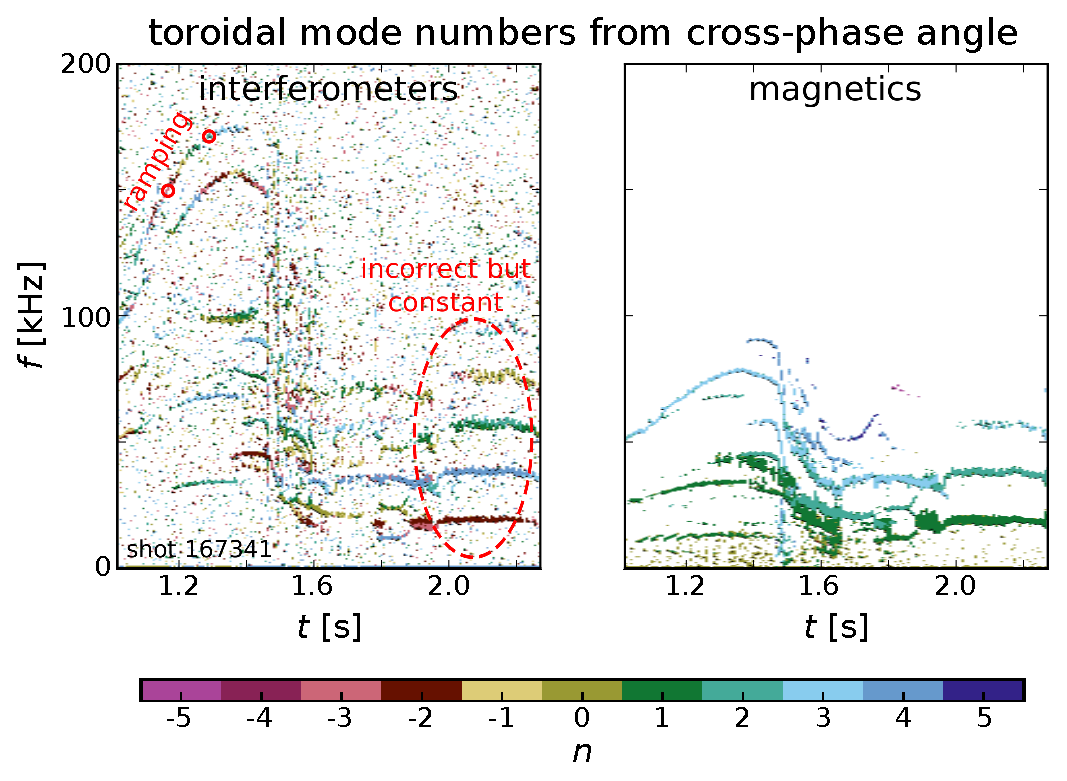
\includegraphics[width = \textwidth]{%
    Chapters/ToroidalCorrelation/figs/mode_numbers_with_uncompensated_time_delay.eps}
  \caption{Computed mode numbers from
    toroidally separated interferometers and magnetics.
    When there is an uncompensated time delay ($\delta t \neq 0$)
    between the two interferometers, as there is here,
    the interferometer-measured mode numbers
    for both constant-frequency and ramping-frequency modes
    are \emph{incorrectly} computed.}
\label{fig:ToroidalCorrelation:uncompensated_time_delay}
\end{figure}

Now, Fig.~\ref{fig:ToroidalCorrelation:uncompensated_time_delay} shows an example
of the computed toroidal mode number spectrum
when using the native time-bases of the V2 and PCI interferometers;
the corresponding magnetics spectrum is shown for comparison.
For $t \lesssim \SI{1.5}{\second}$
the mode frequencies are ramping approximately linearly in time, and
the interferometer-measured mode number is (artificially) ramping in time,
in contrast to the corresponding measurements from magnetics;
application of
(\ref{eq:ToroidalCorrelation:toroidal_mode_number_dt_ramp_rate_lab_frame})
to the \emph{highest-frequency} mode observed by the interferometers yields
$\delta t \approx \SI{-30}{\micro\second}$
($\Delta n = 5$, $\Delta f \approx \SI{20}{\kilo\hertz}$,
as indicated by the positions of the small circular annotations
to the highest frequency mode in
Fig.~\ref{fig:ToroidalCorrelation:uncompensated_time_delay}).
Further, note that the mode number evolution \emph{reverses}
after the mode reaches its peak frequency,
in agreement with the behavior expected from
(\ref{eq:ToroidalCorrelation:toroidal_mode_number_dt_ramp_rate_lab_frame}).
Finally, for $t \gtrsim \SI{2}{\second}$
the mode frequencies are constant, but
the interferometer-measured mode numbers are in disagreement with magnetics.
Naive application of
(\ref{eq:ToroidalCorrelation:toroidal_mode_number_dt_constant_omega})
to the \emph{lowest-frequency} mode at $f \approx \SI{20}{\kilo\hertz}$
yields $\delta t \approx \SI{20}{\micro\second}$
($n_{\text{meas}} = -2$, $n = 1$,
$\omega \approx 2 \pi \cdot \SI{20}{\kilo\hertz}$),
in contrast with the above time-delay estimate
from the linearly ramping mode numbers.
However, as warned above,
$n_{\text{meas}}$ will be \emph{aliased} for ``large'' time delays:
using the above parameters for the lowest-frequency mode,
we see that $|\omega \delta t / \Delta \zeta| \approx 4.8 > n_{\text{Ny}}$,
where $n_{\text{Ny}} = 4$ is the Nyquist mode number
for the $\Delta \zeta = 45^{\circ}$ toroidal separation of the interferometers,
confirming that aliasing has biased our time-delay estimate.
To account for aliasing, we can take $n_{\text{meas}} = -2 \rightarrow 6$, and
application of
(\ref{eq:ToroidalCorrelation:toroidal_mode_number_dt_constant_omega}) yields
$\delta t \approx -\SI{30}{\micro\second}$,
in agreement with the time-delay estimate
from the linearly ramping mode numbers!

The above observations are all consistent with there being an offset
between the native time-bases of the PCI and V2 interferometers, and
the two \emph{independent} measurements of this time offset are in agreement,
with each yielding an offset $\delta t \approx \SI{-30}{\micro\second}$.
Indeed, delaying the PCI signal by $-\SI{30}{\micro\second}$
relative to the V2 signal in software dramatically improves
the agreement between the interferometer and magnetics mode number spectra.
By scanning $\delta t$ about $-\SI{30}{\micro\second}$ and
noting when discrepancy with magnetics began to creep back into
the interferometer-measured mode spectrum,
the upper and lower bounds of $\delta t$ were found;
the best estimate for $\delta t$ was then taken as the midpoint
between these upper and lower bounds, which was found to be
\begin{equation}
  \delta t = -\SI{32}{\micro\second}
  \label{eq:ToroidalCorrelation:time_delay}
\end{equation}
That is, the native PCI-interferometer's time base \emph{leads}
the native V2 time base by $\SI{32}{\micro\second}$.
Delaying the PCI-interferometer by $\SI{32}{\micro\second}$ (in software)
relative to the V2 interferometer yields the mode number spectrum
shown in Fig.~\ref{fig:ToroidalCorrelation:compensated_time_delay}.
Note that both
Fig.~\ref{fig:ToroidalCorrelation:uncompensated_time_delay} and
Fig.~\ref{fig:ToroidalCorrelation:compensated_time_delay}
correspond to shot 167341, and
the only difference in the interferometer-measured mode number spectrum
between the two figures results from the compensation of the time delay
between the native time bases of the two interferometers.

\textcolor{red}{Note that additional measurements are needed
to determine which clock is correct in the \emph{absolute} sense.
For example, we can try digitizing a trigger signal and
comparing the digitized time of the trigger to the ``nominal'' trigger time
to determine the offset of our digitizer from the DIII-D clock.}

\begin{figure}
  \centering
  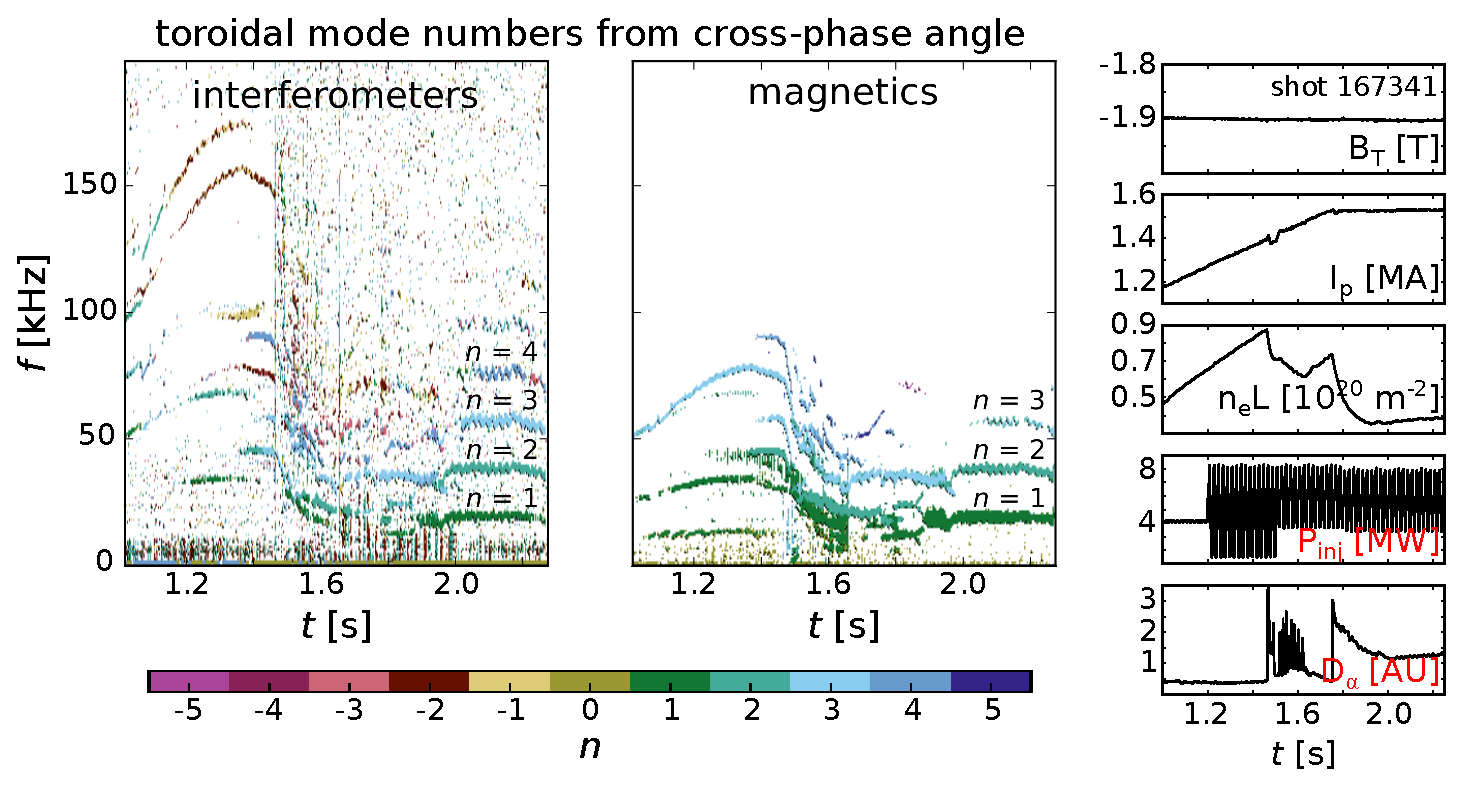
\includegraphics[width = \textwidth]{%
    Chapters/ToroidalCorrelation/figs/magnetics_and_interferometer_mode_numbers_167341.eps}
  \caption{Computed mode numbers from
    toroidally separated interferometers and magnetics.
    Here, the PCI-interferometer signal has been delayed by
    $\SI{32}{\micro\second}$ relative to the V2 signal
    to account for the time offset between each system's native time base.
    Note that the agreement with magnetics is excellent and that
    the mode numbers of the ramping-frequency modes are no longer
    artificially ramping;
    this is an enormous improvement over the corresponding
    uncompensated interferometer-measured spectrum in
    Fig.~\ref{fig:ToroidalCorrelation:uncompensated_time_delay}.}
\label{fig:ToroidalCorrelation:compensated_time_delay}
\end{figure}


\subsection{Radial offset}
The V2 and PCI interferometer beam paths have a slight radial offset
($\Delta R = \SI{4}{\centi\meter}$ with
$R_{\text{V2}} = \SI{1.94}{\meter}$ and $R_{\text{PCI}} = \SI{1.98}{\meter}$).
Thus, $\alpha_{12} = n(\zeta_2 - \zeta_1) + [\sigma(R_2) - \sigma(R_1)]$.
Recall that $\sigma_F$ is a complicated function of
the beam's major radial location,
the mode structure,
the equilibrium density profile, and
the plasma geometry.
However, the \emph{dominant} effect of such a radial offset
is attributable to the relative phase of $\vect{\xi}$
at the two radial locations:
\begin{equation}
  \sigma(R_2) - \sigma(R_1)
  \approx
  \begin{cases}
    0, & \quad \text{$\vect{\xi}(R_1)$ and $\vect{\xi}(R_2)$ in-phase} \\
    \pi, & \quad \text{$\vect{\xi}(R_1)$ and $\vect{\xi}(R_2)$ out-of-phase}
  \end{cases}
  \notag
\end{equation}
If $\vect{\xi}(R_1)$ and $\vect{\xi}(R_2)$ are in-phase,
then application of (\ref{eq:ToroidalCorrelation:toroidal_mode_number_ideal})
will yield the correct mode number.
However, if $\vect{\xi}(R_1)$ and $\vect{\xi}(R_2)$ are out-of-phase,
then application of (\ref{eq:ToroidalCorrelation:toroidal_mode_number_ideal})
will yield a measured mode number $n_{\text{meas}}$
\begin{equation}
  n_{\text{meas}}
  =
  \begin{cases}
    n + n_{\text{Ny}}, & \quad n \leq 0 \\
    n - n_{\text{Ny}}, & \quad n > 0
  \end{cases}
  \label{eq:ToroidalCorrelation:toroidal_mode_number_radially_out_of_phase}
\end{equation}
where $n_{\text{Ny}} \equiv \pi / \Delta \zeta$
is the Nyquist toroidal mode number, and
the $n > 0$ case results from \emph{aliasing}
(that is, $n + n_{\text{Ny}} \rightarrow n - n_{\text{Ny}}$
when $n > 0$ because of aliasing).
Lacking additional measurements or some type of forward modeling,
this incorrect mode-number identification may go undiagnosed.
However, if $\vect{\xi}(R)$ evolves such that
$\vect{\xi}(R_1)$ and $\vect{\xi}(R_2)$ transition
from being in-phase to being out-of-phase (or vice versa),
the measured mode number will ``flip'';
an example of this mode-number ``flipping''
is shown in Fig.~\ref{fig:ToroidalCorrelation:mode_number_flips}.
Further effects of the radial offset can be investigated
via e.g.\ forward modeling and synthetic diagnostics.

\begin{figure}
  \centering
  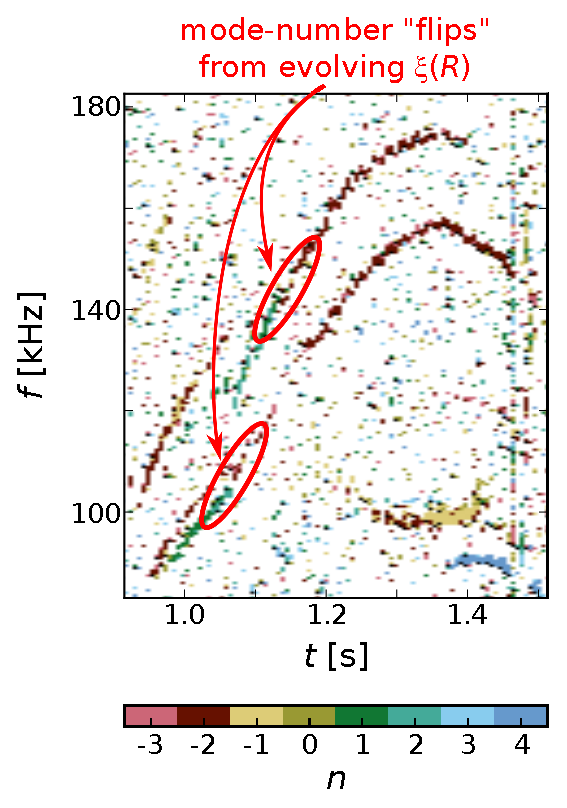
\includegraphics[width = 0.5 \textwidth]{%
    Chapters/ToroidalCorrelation/figs/phase_flips_167341.eps}
  \caption{Due to the small radial offset ($\Delta R = \SI{4}{\centi\meter}$)
    between the V2 and PCI interferometers,
    changes in the radial structure of a mode
    can result in ``flipping'' of the interferometer-measured mode number.
    Here, the mode number flips from $n = 2$ to $n = -2$,
    consistent with
    (\ref{eq:ToroidalCorrelation:toroidal_mode_number_radially_out_of_phase}).
    Lacking additional measurements or some type of forward modeling,
    it is impossible to determine if the mode is truly $n = 2$ or $n = -2$.
    Note that these modes exceed the typical bandwidth of magnetics, however,
    so even identification as $n = \pm 2$ \emph{is} an improvement!}
\label{fig:ToroidalCorrelation:mode_number_flips}
\end{figure}


\section{Example mode number spectra}

\begin{figure}[h!]
  \centering
  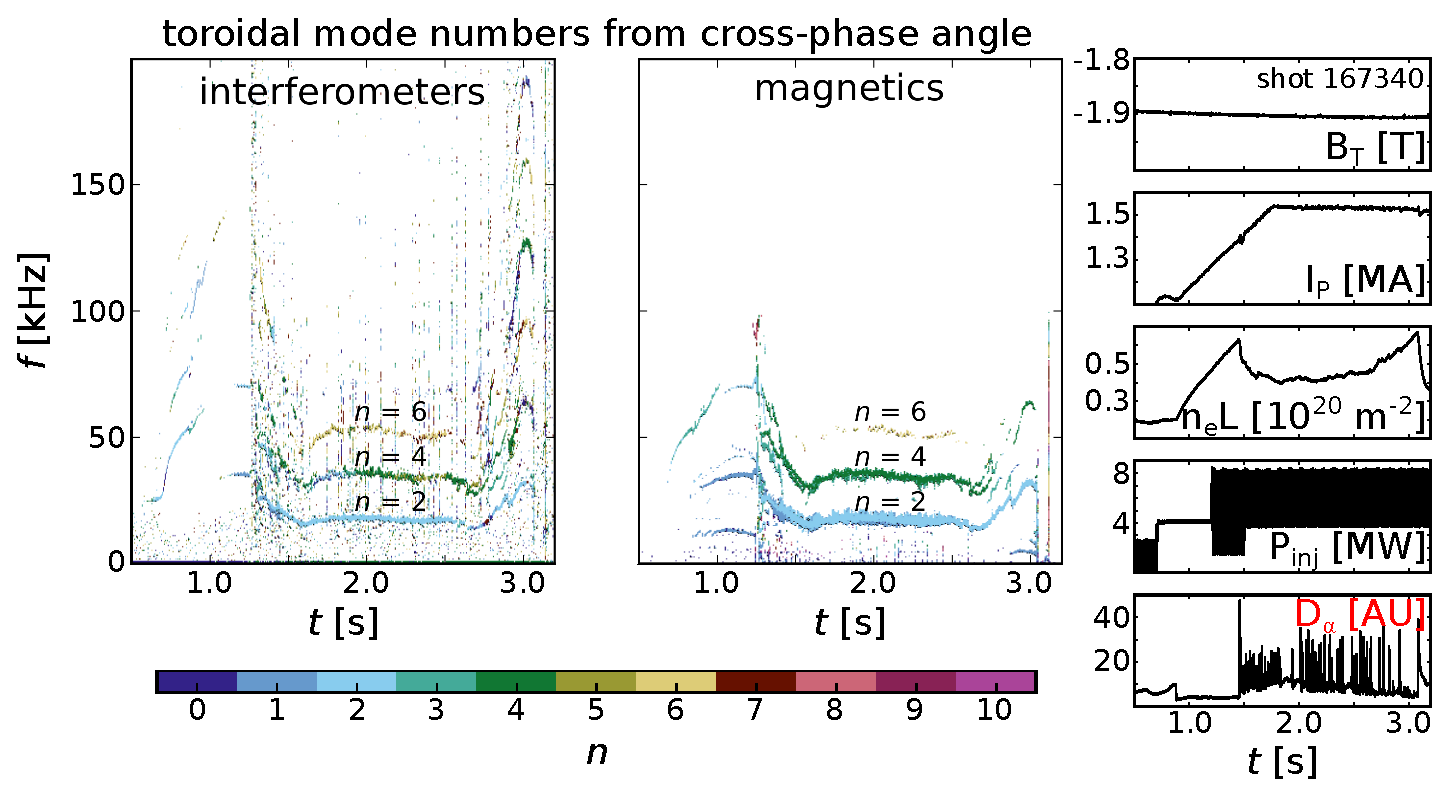
\includegraphics[width = \textwidth]{%
    Chapters/ToroidalCorrelation/figs/magnetics_and_interferometer_mode_numbers_167340.eps}
  \caption{Another example of excellent agreement between the
    interferometer and magnetics mode number spectra. Note that
    the interferometers additionally see modes \emph{invisible} to magnetics.
    Here,the modes were \emph{assumed} to be rotating
    in the ``positive'' direction
    (i.e.\ counterclockwise when viewing the torus from above,
    as this corresponds to the direction of dominant torque injection)
    such that we can discriminate $0 \leq n < 8$
    (rather than the typical $-4 < n \leq 4$).}
\label{fig:ToroidalCorrelation:magnetics_corroboration_2}
\end{figure}

\begin{figure}[h!]
  \centering
  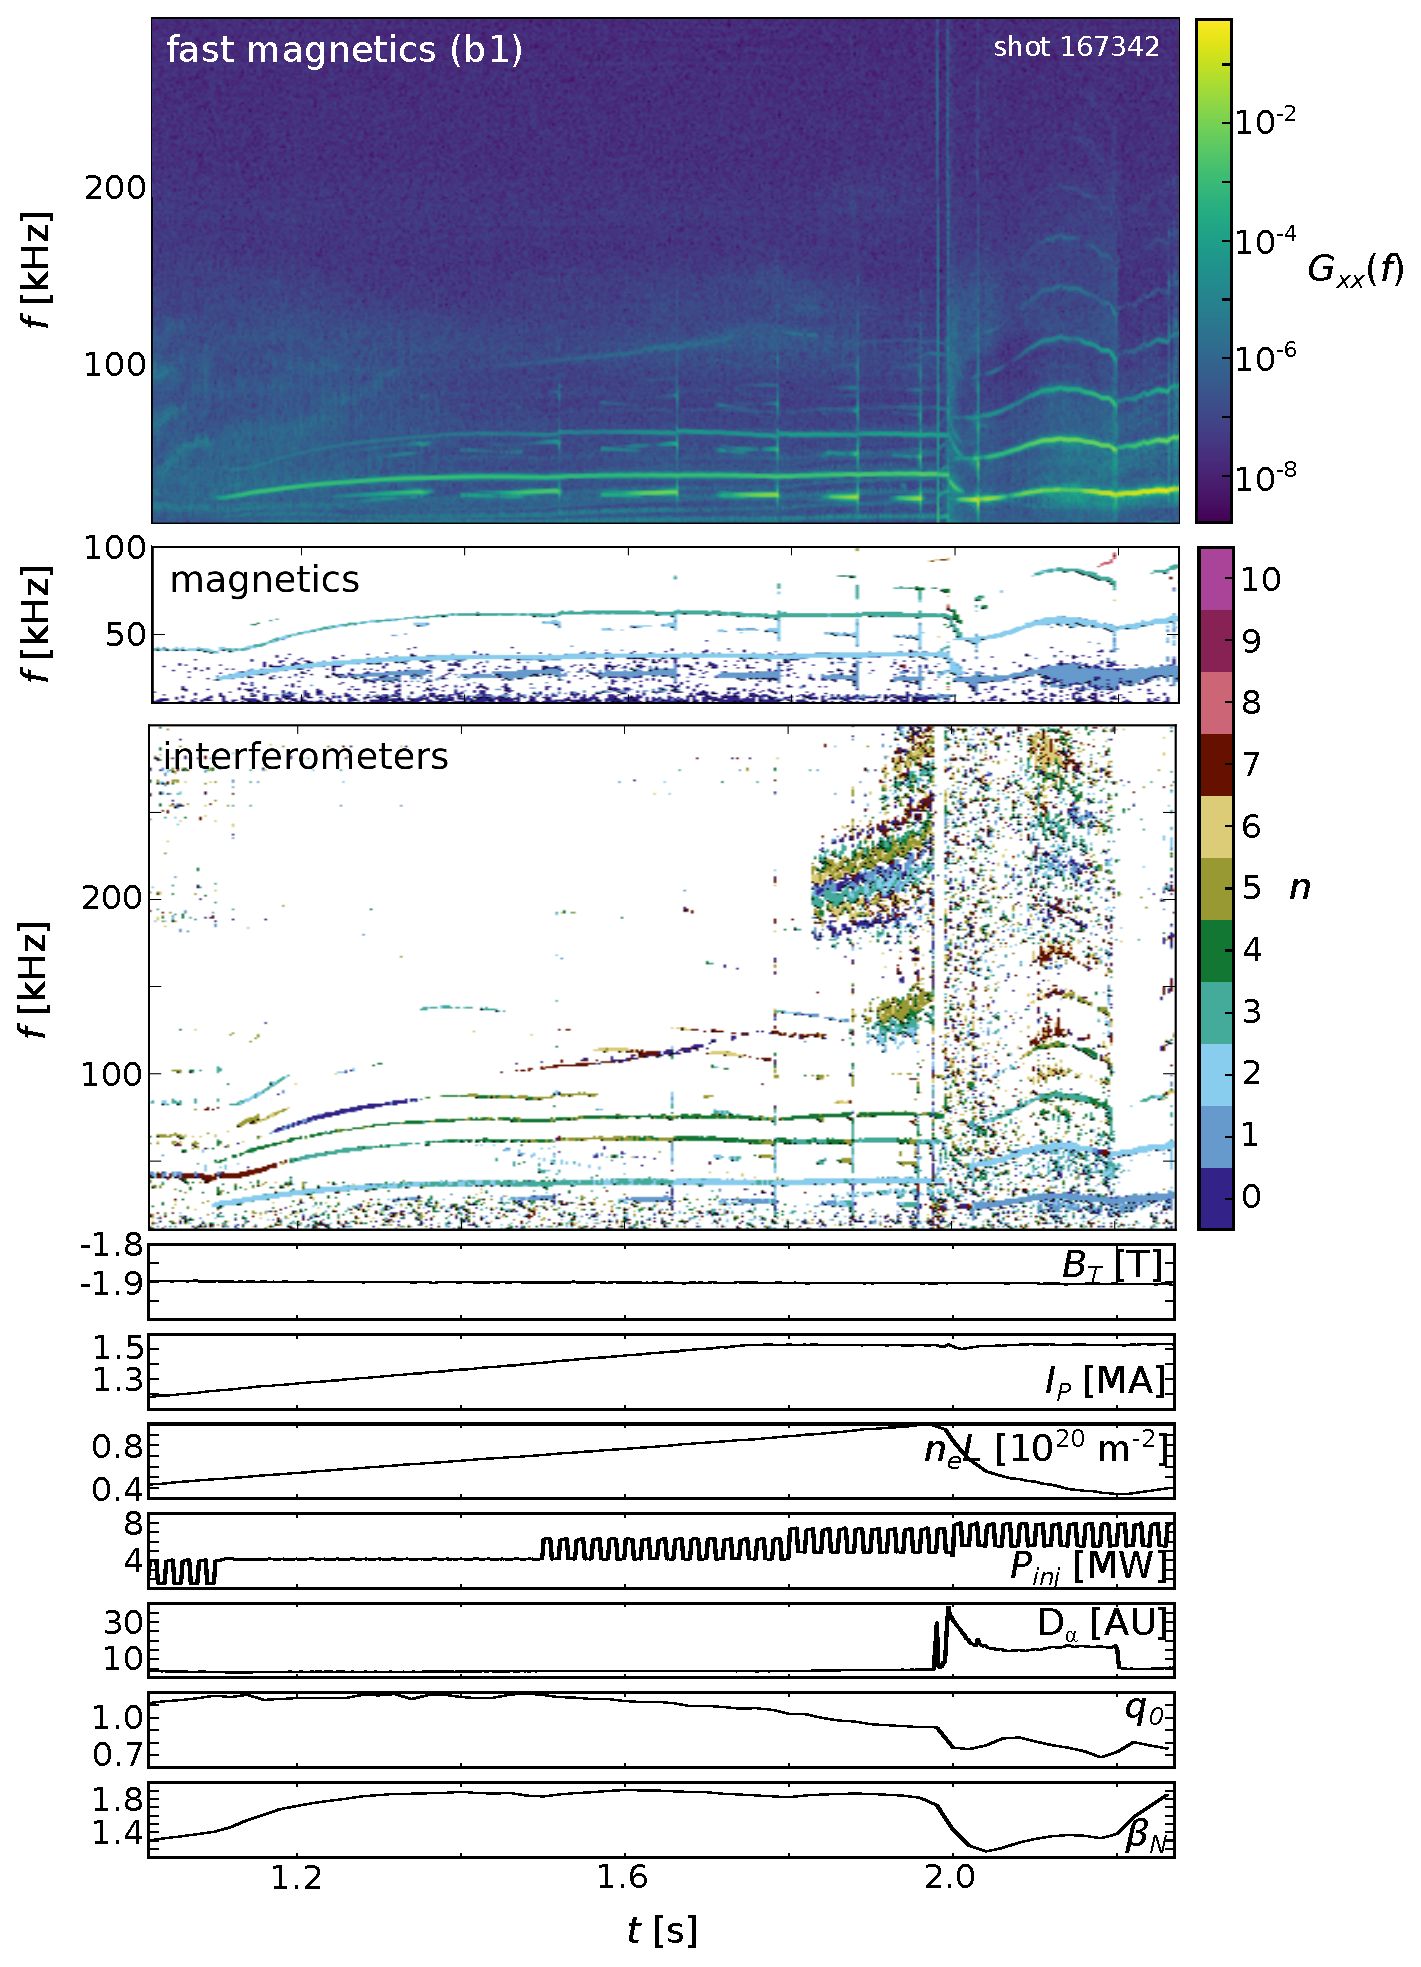
\includegraphics[width = 0.8 \textwidth]{%
    Chapters/ToroidalCorrelation/figs/core_localized_167342.eps}
  \caption{Between $1.8 \leq t \, [\text{s}] \leq 2.2$,
    the correlated interferometers measure fluctuations
    (Alfv\'{e}n eigenmodes?) that are \emph{invisible} to magnetics.
    This suggests that the modes are \emph{core-localized} and
    that the correlated interferometers are indeed capable
    of measuring core-localized MHD!
    (Note that the fast magnetic probes have a \SI{1}{\mega\hertz} bandwidth,
    but they do not have significant toroidal separation,
    preventing accurate measurement of toroidal mode numbers).}
\label{fig:ToroidalCorrelation:core_localized}
\end{figure}

\begin{figure}[h!]
  \centering
  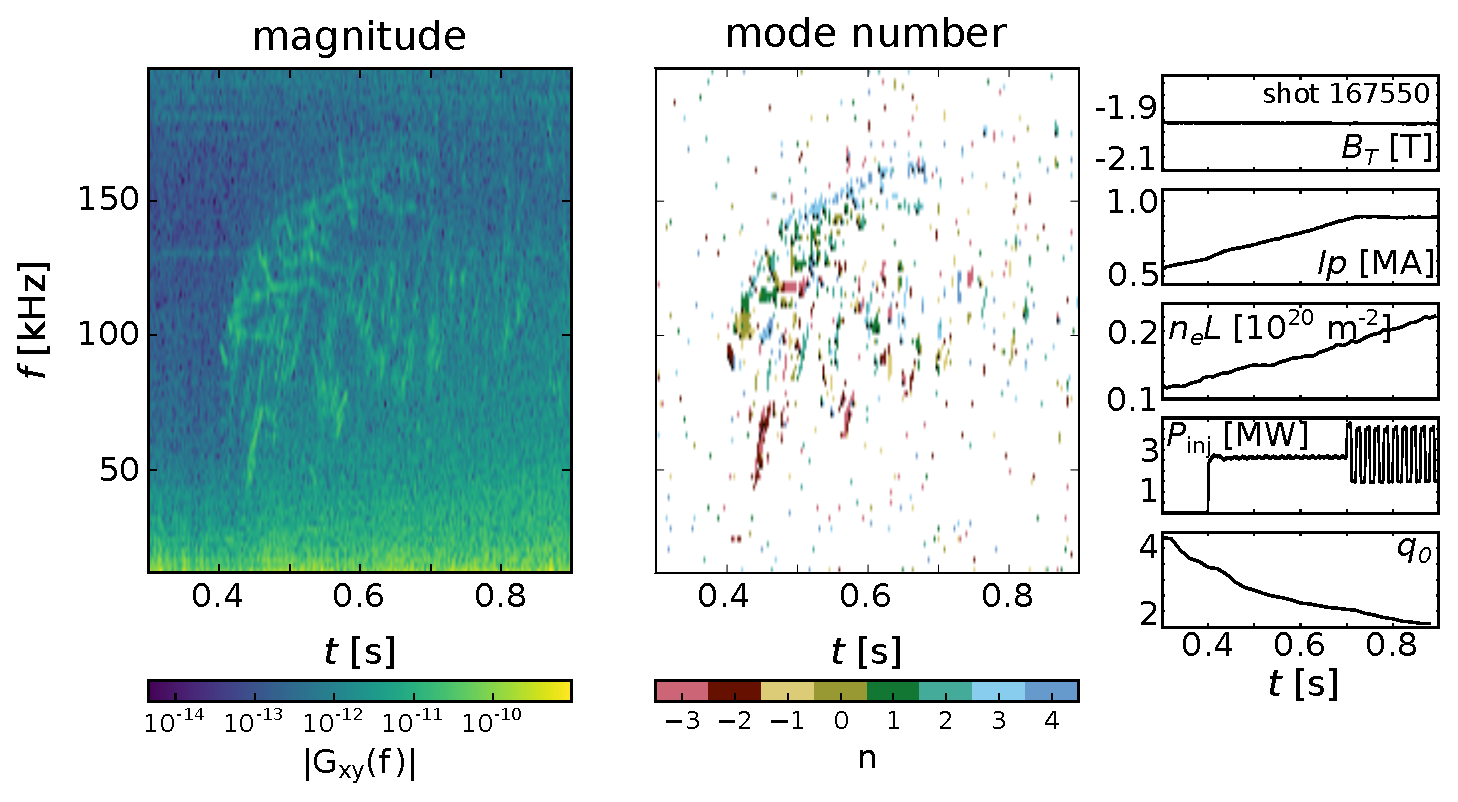
\includegraphics[width = \textwidth]{%
    Chapters/ToroidalCorrelation/figs/AEs_167550.eps}
  \caption{Alfv\'{e}n eigenmodes (?) visible
    on the correlated interferometers.
    These modes are not readily visible on magnetics.}
\label{fig:ToroidalCorrelation:AEs}
\end{figure}

\begin{figure}[h!]
  \centering
  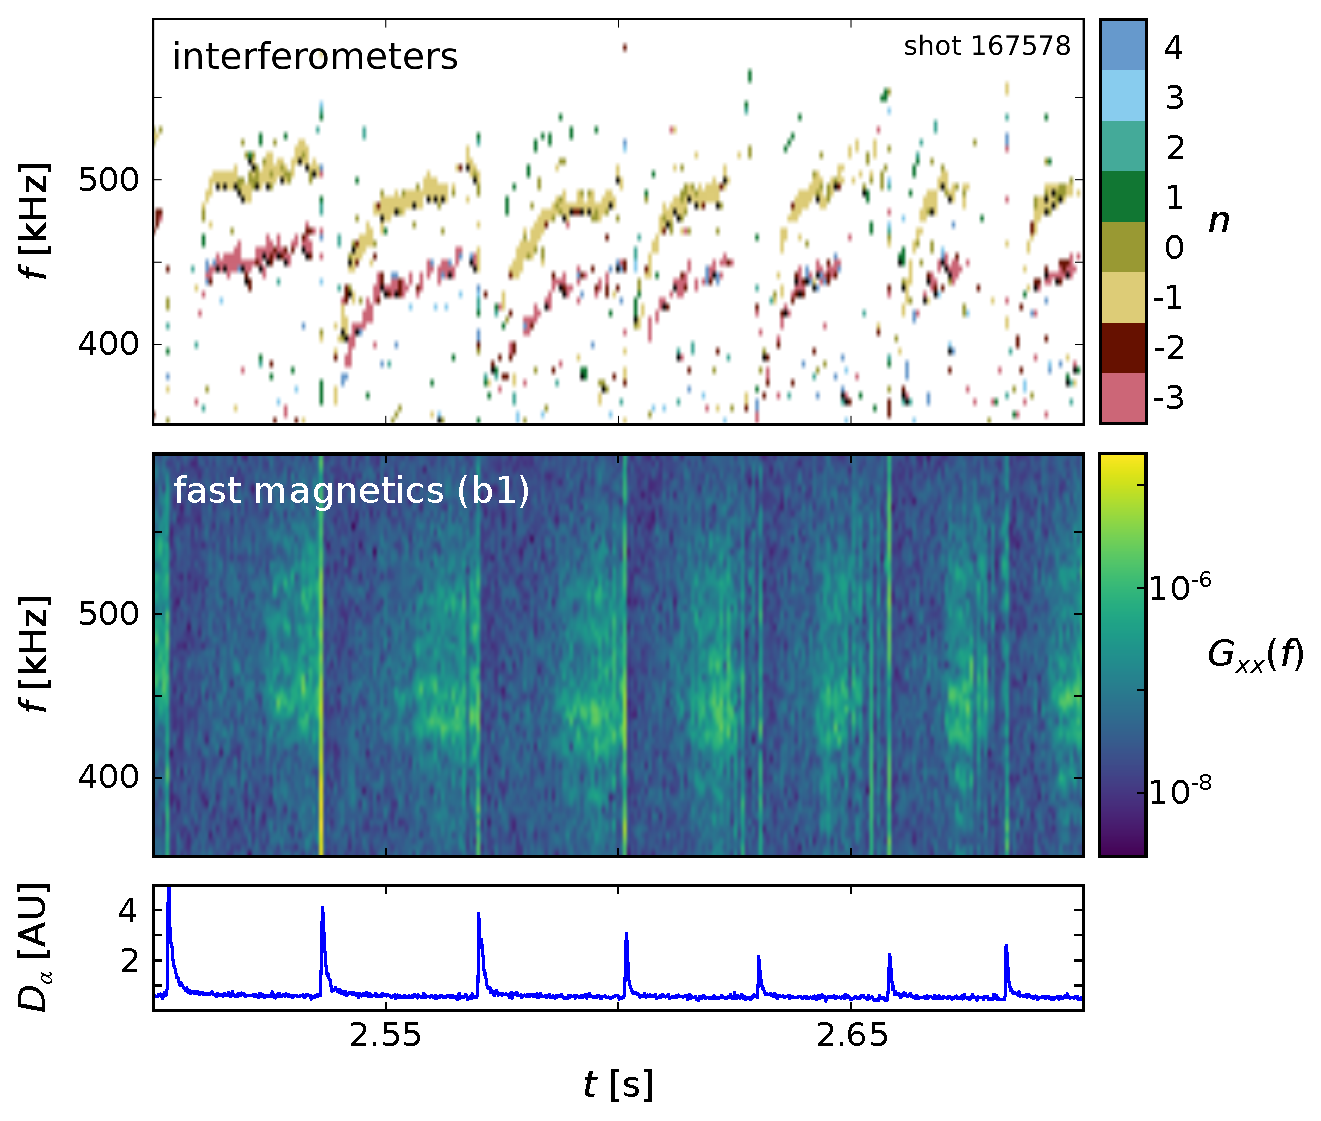
\includegraphics[width = 0.7 \textwidth]{%
    Chapters/ToroidalCorrelation/figs/interELM_fast_167578.eps}
  \caption{Inter-ELM fluctuations as measured by
    the correlated interferometers and fast magnetics.
    The mode frequency ramps early in the inter-ELM window before saturating;
    the magnetic component of the fluctuation only appears \emph{after}
    the mode frequency has saturated --- fascinating!
    (Note that the fast magnetic probes have a \SI{1}{\mega\hertz} bandwidth,
    but they do not have significant toroidal separation,
    preventing accurate measurement of toroidal mode numbers).
    The drive and significance of such fluctuations is not known, but
    they do \emph{not} occur in every ELMy discharge.}
\label{fig:ToroidalCorrelation:interELM_fast}
\end{figure}

\begin{figure}[h!]
  \centering
  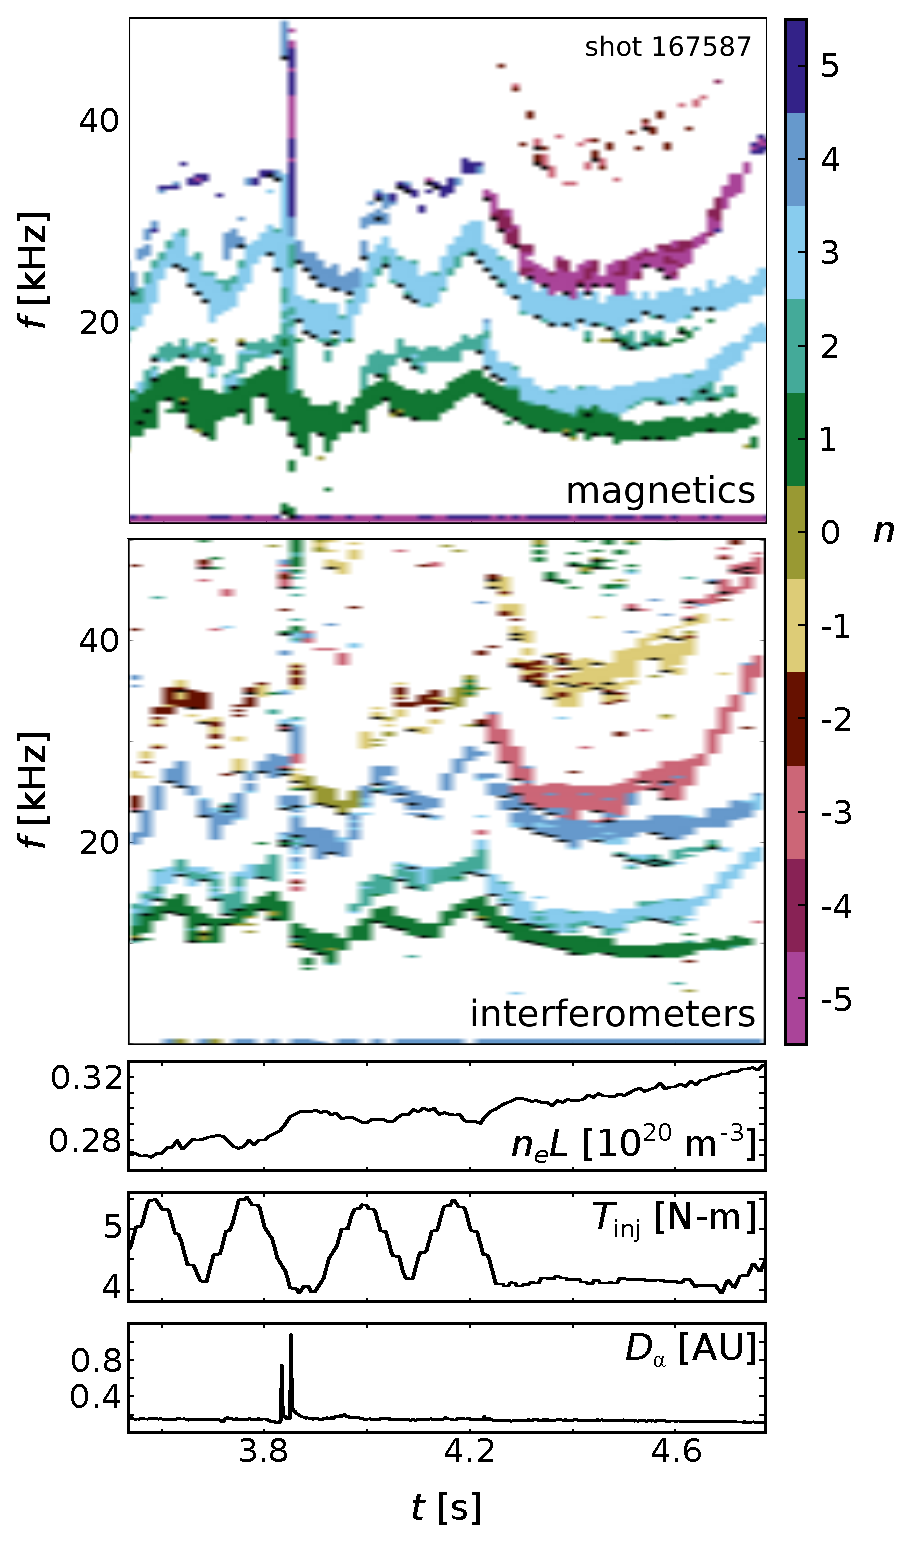
\includegraphics[width = 0.5 \textwidth]{%
    Chapters/ToroidalCorrelation/figs/EHO_167587.eps}
  \caption{The magnetics and interferometers both see the
    edge harmonic oscillation (EHO), which is responsible for
    flushing impurities from quiescent H-mode (QH-mode) plasmas.
    Below \SI{20}{\kilo\hertz}, the magnetics and interferometers
    both measure the same toroidal mode numbers; however,
    above \SI{20}{\kilo\hertz}, the measured mode numbers differ,
    likely due to a combination of aliasing and the small radial offset
    of the two interferometer beams.}
\label{fig:ToroidalCorrelation:EHO}
\end{figure}

\begin{figure}[h!]
  \centering
  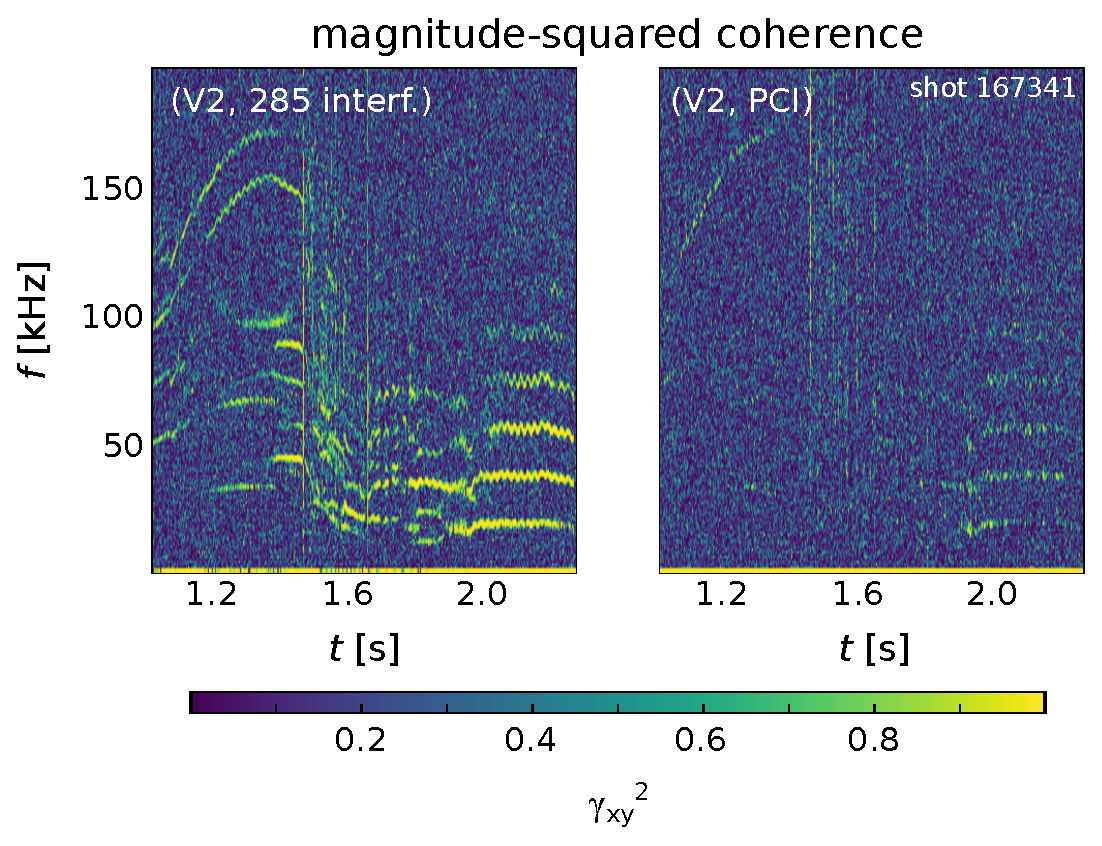
\includegraphics[width = 0.75 \textwidth]{%
    Chapters/ToroidalCorrelation/figs/interferometer_vs_PCI_coherence.eps}
  \caption[%
    Inability to correlate V2 and PCI]{%
      The magnitude-squared coherence $\gamma_{xy}^2$ between
      the V2 and 285 interferometers (left) and
      between the V2 interferometer and PCI (right).
      The high coherence between the V2 and 285 interferometers
      allows accurate measurement of toroidal mode numbers,
      as demonstrated by the corresponding mode number spectrum
      displayed in Fig.~\ref{fig:ToroidalCorrelation:compensated_time_delay},
      whereas the poor coherence between the V2 and PCI
      prevents such measurements.
      (Note that ``285 interferometer'' refers to
      the newly installed interferometer channel of the PCI).}
\label{fig:ToroidalCorrelation:PCI_coherence}
\end{figure}


\bibliographystyle{plainurl}
\bibliography{references}
